\section{多元中心极限定理}
\label{sec:clt-multivariate}

掷$n$次骰子，记下六个面各出现了多少次；或者同时测量一批零件的长度和重量。这时每次观测是一个向量，平均也是向量。各分量的平均分别近似高斯还不够，我们还想知道它们的偏差怎样联合分布：长度偏大时重量是否也偏大，六个频率之和恒为一这一约束又怎样体现在极限里。

设$\bm{X}_1,\bm{X}_2,\dots$是$\mathbb{R}^{d}$中独立同分布的随机向量，维数$d$固定，$\mathbb{E}[\lVert\bm{X}_1\rVert_2^2]<\infty$。记均值向量为$\bm{\mu}$，协方差矩阵为$\bm{\Sigma}$（粗体大写表示$d\times d$矩阵），样本平均为
\[
 \bar{\bm{X}}_n=\frac1n\sum_{i=1}^{n}\bm{X}_i .
\]
要研究的对象是$\sqrt{n}(\bar{\bm{X}}_n-\bm{\mu})$。这里不除以标准差：向量没有单一的标准差，$\bm{\Sigma}$还可能不可逆。极限中会直接出现$\bm{\Sigma}$本身。

\paragraph{两枚硬币的例子}
设$\xi,\eta$独立，各以$1/2$的概率取$\pm1$，令$\bm{X}=(\xi,\ \xi+\eta)^{\top}$。两个分量共享$\xi$，所以正相关。直接计算，$\bm{\mu}=\bm{0}$，
\[
 \operatorname{Var}(\xi)=1,\qquad \operatorname{Var}(\xi+\eta)=2,\qquad \operatorname{Cov}(\xi,\xi+\eta)=\operatorname{Var}(\xi)=1 ,
\]
即
\[
 \bm{\Sigma}=\begin{bmatrix}1&1\\1&2\end{bmatrix} .
\]
本节还用一个退化的对照：$\bm{X}=(\xi,\ 2\xi)^{\top}$，协方差矩阵的各元为$1,2,2,4$，行列式为零。

\subsection{方向投影}
\label{sec:clt-projection}

向量的分布不容易直接处理，可以先把它投到各个方向上，变成标量问题。固定$\bm{a}\in\mathbb{R}^{d}$，投影$\bm{a}^{\top}\bm{X}_i$是独立同分布的实随机变量。由第~\ref{chap:random-vectors}章的均值与协方差的线性规则，
\[
 \mathbb{E}[\bm{a}^{\top}\bm{X}_i]=\bm{a}^{\top}\bm{\mu},\qquad \operatorname{Var}(\bm{a}^{\top}\bm{X}_i)=\bm{a}^{\top}\bm{\Sigma}\bm{a} .
\]
投影与平均可以交换，$\bm{a}^{\top}\sqrt{n}(\bar{\bm{X}}_n-\bm{\mu})$正是投影序列的$\sqrt{n}$倍平均偏差。按$\bm{a}^{\top}\bm{\Sigma}\bm{a}$是否为零分两种情形。

\paragraph{正方差方向}
若$\bm{a}^{\top}\bm{\Sigma}\bm{a}>0$，投影序列满足定理~\ref{thm:clt-iid}的全部条件，所以
\[
 \frac{\sqrt{n}\,\bm{a}^{\top}(\bar{\bm{X}}_n-\bm{\mu})}{\sqrt{\bm{a}^{\top}\bm{\Sigma}\bm{a}}}\xrightarrow{\mathrm{d}}\mathcal{N}(0,1) .
\]
记左边为$W_n$，再乘回常数$c=\sqrt{\bm{a}^{\top}\bm{\Sigma}\bm{a}}>0$。对每个$x$，
\[
 \mathbb{P}(cW_n\leq x)=\mathbb{P}\Bigl(W_n\leq\frac{x}{c}\Bigr)\to\Phi\Bigl(\frac{x}{c}\Bigr) ,
\]
右边是$\mathcal{N}(0,c^2)$的分布函数。于是
\begin{equation}
 \sqrt{n}\,\bm{a}^{\top}(\bar{\bm{X}}_n-\bm{\mu})\xrightarrow{\mathrm{d}}\mathcal{N}(0,\bm{a}^{\top}\bm{\Sigma}\bm{a}) .
 \label{eq:clt-projection}
\end{equation}

\paragraph{零方差方向}
若$\bm{a}^{\top}\bm{\Sigma}\bm{a}=0$，标准化要除以零，不能套用。这时$\bm{a}^{\top}(\bm{X}_i-\bm{\mu})$均值为零、方差为零，几乎必然等于零。于是对每个$n$，
\[
 \sqrt{n}\,\bm{a}^{\top}(\bar{\bm{X}}_n-\bm{\mu})=\frac{1}{\sqrt{n}}\sum_{i=1}^{n}\bm{a}^{\top}(\bm{X}_i-\bm{\mu})=0\quad\text{几乎必然} .
\]
它的分布恒为$0$处的单点分布，当然依分布收敛到这个单点分布。按第~\ref{sec:clt-standardization}节的约定，单点分布就是$\mathcal{N}(0,0)$，所以式~\eqref{eq:clt-projection}在零方差方向也成立。

\paragraph{两枚硬币的投影}
对$\bm{X}=(\xi,\ \xi+\eta)^{\top}$，三个方向上的极限方差分别是
\[
 \bm{a}=(1,0)^{\top}:\ 1,\qquad \bm{a}=(0,1)^{\top}:\ 2,\qquad \bm{a}=\tfrac{1}{\sqrt2}(1,-1)^{\top}:\ \tfrac12(1-2+2)=\tfrac12 .
\]
最后一个方向是两分量之差，$\xi-(\xi+\eta)=-\eta$，方差本来就是$1$，除以$(\sqrt2)^2$后为$1/2$。图~\ref{fig:clt-projections}用$n=100$、$1500$次重复模拟检验这三个结论，三个直方图的样本方差分别为$0.98$、$1.99$、$0.47$。

\begin{BookInlineFigure}
 \centering
 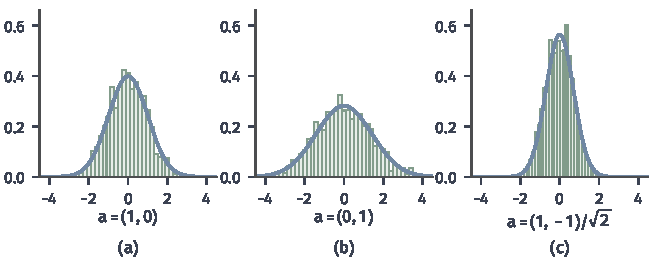
\includegraphics[width=112mm]{figures/07-probability/03-probability-limits/matplotlib/clt-projections/figure.pdf}
 \caption{$\bm{X}=(\xi,\xi+\eta)^{\top}$、$n=100$时$\bm{a}^{\top}\sqrt{n}\,\bar{\bm{X}}_n$的直方图（浅绿，$1500$次重复，种子$3$，每个格点一个柱）与$\mathcal{N}(0,\bm{a}^{\top}\bm{\Sigma}\bm{a})$的密度（蓝）。(a)$\bm{a}=(1,0)^{\top}$，方差$1$；(b)$\bm{a}=(0,1)^{\top}$，方差$2$；(c)$\bm{a}=(1,-1)^{\top}/\sqrt2$，方差$1/2$。}
 \label{fig:clt-projections}
\end{BookInlineFigure}

对退化的$\bm{X}=(\xi,\ 2\xi)^{\top}$，方向$\bm{a}=(2,-1)^{\top}$给出$\bm{a}^{\top}\bm{X}=2\xi-2\xi=0$，这是零方差方向；与它垂直的方向$(1,2)^{\top}/\sqrt5$上，投影是$\sqrt5\,\xi$，方差为$5$。

\subsection{联合高斯极限}
\label{sec:clt-joint}

每个方向上的极限都是高斯的，方差由同一个矩阵$\bm{\Sigma}$按$\bm{a}^{\top}\bm{\Sigma}\bm{a}$给出。第~\ref{chap:multivariate-distributions}章说明，若$\bm{W}\sim\mathcal{N}(\bm{0},\bm{\Sigma})$，则对每个$\bm{a}$，
\begin{equation}
 \bm{a}^{\top}\bm{W}\sim\mathcal{N}(0,\bm{a}^{\top}\bm{\Sigma}\bm{a}) .
 \label{eq:clt-gauss-projection}
\end{equation}
所以各方向的极限恰好是同一个高斯向量$\bm{W}$的各个投影。Cramér--Wold判据说，在固定维数中，所有方向的投影依分布收敛到同一个向量的投影，就足以推出向量本身依分布收敛。

\begin{theorem}[多元中心极限定理]
\label{thm:clt-multivariate}
设$\bm{X}_1,\bm{X}_2,\dots$是$\mathbb{R}^{d}$中独立同分布的随机向量，$\mathbb{E}[\lVert\bm{X}_1\rVert_2^2]<\infty$，均值为$\bm{\mu}$，协方差矩阵为$\bm{\Sigma}$。则
\begin{equation}
 \sqrt{n}\,(\bar{\bm{X}}_n-\bm{\mu})\xrightarrow{\mathrm{d}}\mathcal{N}(\bm{0},\bm{\Sigma}) .
 \label{eq:clt-multivariate}
\end{equation}
\end{theorem}

这个结论称为\term{多元中心极限定理}（multivariate central limit theorem）。

\begin{proof}
设$\bm{W}\sim\mathcal{N}(\bm{0},\bm{\Sigma})$。对每个$\bm{a}\in\mathbb{R}^{d}$，由式~\eqref{eq:clt-projection}，投影$\bm{a}^{\top}\sqrt{n}(\bar{\bm{X}}_n-\bm{\mu})$依分布收敛到$\mathcal{N}(0,\bm{a}^{\top}\bm{\Sigma}\bm{a})$，正方差与零方差方向都包括在内。由式~\eqref{eq:clt-gauss-projection}，这个极限就是$\bm{a}^{\top}\bm{W}$的分布。由Cramér--Wold判据，$\sqrt{n}(\bar{\bm{X}}_n-\bm{\mu})\xrightarrow{\mathrm{d}}\bm{W}$。
\end{proof}

\paragraph{为什么要看所有方向}
只看坐标方向，得到的是每个分量各自的极限，即边缘分布的收敛。第~\ref{chap:weak-convergence-of-distributions}章说明，边缘收敛不能确定分量之间的配对方式。两枚硬币的例子里，两个分量的极限分别是$\mathcal{N}(0,1)$与$\mathcal{N}(0,2)$；它们是相互独立，还是相关系数为$1/\sqrt2$，只有斜方向（例如图~\ref{fig:clt-projections}(c)）的方差能分辨：独立时差的方差应是$\frac12(1+2)=\frac32$，实际是$\frac12$。定理的证明用到了全部方向，所以得到的是联合极限，相关结构由$\bm{\Sigma}$的非对角元保留下来。

图~\ref{fig:clt-bivariate-scatter}(a)把同一批模拟的点$\sqrt{n}\,\bar{\bm{X}}_n$画在平面上，点云沿主对角方向拉长。$\mathcal{N}(\bm{0},\bm{\Sigma})$在马氏距离$1$与$2$以内的概率是$1-\mathrm{e}^{-1/2}\approx0.393$与$1-\mathrm{e}^{-2}\approx0.865$，模拟点落在这两个椭圆内（含边界）的比例是$0.398$与$0.885$，边界上的格点使后者略偏大。点排成格子，因为$n=100$时每个分量只取间距为$0.2$的格点值；依分布收敛并不要求有限$n$的分布有密度。

\begin{BookInlineFigure}
 \centering
 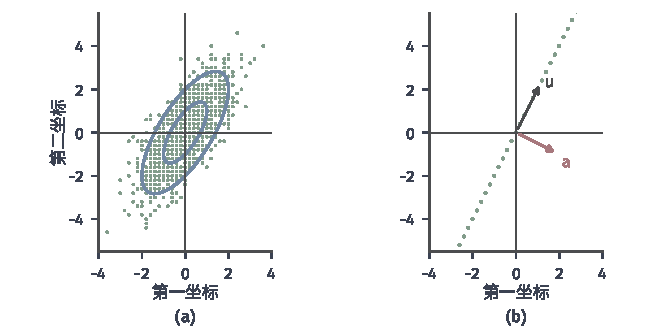
\includegraphics[width=112mm]{figures/07-probability/03-probability-limits/matplotlib/clt-bivariate-scatter/figure.pdf}
 \caption{$n=100$时$\sqrt{n}\,\bar{\bm{X}}_n$的$1500$个模拟点（绿，种子$3$）。(a)$\bm{X}=(\xi,\xi+\eta)^{\top}$，蓝色椭圆是$\mathcal{N}(\bm{0},\bm{\Sigma})$在马氏距离$1$与$2$处的等高线；(b)$\bm{X}=(\xi,2\xi)^{\top}$，点全部落在直线$y=2x$上，红色箭头$\bm{a}$是零方差方向$(2,-1)^{\top}/\sqrt5$，灰色箭头$\bm{u}$是直线方向$(1,2)^{\top}/\sqrt5$。}
 \label{fig:clt-bivariate-scatter}
\end{BookInlineFigure}

\paragraph{奇异的协方差矩阵}
定理不要求$\bm{\Sigma}$可逆。退化例子中$\bm{\Sigma}$的秩为一，极限$\mathcal{N}(\bm{0},\bm{\Sigma})$是第~\ref{chap:multivariate-distributions}章的退化高斯分布，全部质量在直线$\{t(1,2)^{\top}:t\in\mathbb{R}\}$上，在平面上没有密度。图~\ref{fig:clt-bivariate-scatter}(b)中有限$n$的点也都在这条直线上。若要写出标准化的形式$\bm{\Sigma}^{-1/2}\sqrt{n}(\bar{\bm{X}}_n-\bm{\mu})$，就必须假设$\bm{\Sigma}$可逆；式~\eqref{eq:clt-multivariate}的写法避开了这个假设。

\paragraph{骰子的频率}
掷一枚均匀骰子$n$次，令$\bm{X}_i\in\mathbb{R}^{6}$是第$i$次结果的示性向量：出现第$j$面时第$j$个分量为$1$，其余为$0$。$\bar{\bm{X}}_n$就是六个面的频率向量，$n\bar{\bm{X}}_n\sim\operatorname{Mult}(n,\bm{p})$，$\bm{p}=\frac16\bm{1}$。由$X_{i,j}X_{i,k}=0$（$j\neq k$）与$X_{i,j}^2=X_{i,j}$，
\[
 \bm{\Sigma}=\operatorname{diag}(\bm{p})-\bm{p}\bm{p}^{\top},\qquad \Sigma_{j,j}=\frac16-\frac1{36}=\frac{5}{36},\qquad \Sigma_{j,k}=-\frac{1}{36}\ (j\neq k) .
\]
由定理~\ref{thm:clt-multivariate}，$\sqrt{n}(\bar{\bm{X}}_n-\bm{p})\xrightarrow{\mathrm{d}}\mathcal{N}(\bm{0},\bm{\Sigma})$。频率之和恒为一，所以$\bm{1}^{\top}(\bm{X}_i-\bm{p})=0$，$\bm{1}$是零方差方向，$\bm{\Sigma}\bm{1}=\bm{0}$。极限分布集中在“六个偏差之和为零”的五维子空间上，各频率偏差之间是负相关：一个面出现得多，其余的面就只能少。

\paragraph{维数固定}
定理中的$d$在$n\to\infty$时保持不变。它不说明维数随样本量一同增长时会怎样，也不涉及部分和作为$n$的函数、整条随机路径的极限形状；后者需要在函数空间中讨论收敛，超出了有限维概率极限的范围。
